\section{VLBI}


\section{DORIS}
DORIS (Doppler Orbitography and Radiopositioning Integrated by Satellite) jest francuskim cywilnym systemem montowanym 
na satelitach służącym głównie do precyzyjnego wyznaczania orbit sztucznych satelitów Ziemi oraz pozycjonowania aktywnych stacji referencyjnych.
Zaprojektowany przez Francuską agencję kosmiczną Cnes, system bazuje na efekcie Doplera zmiany częstotliwości rejestrowanej przez odbiornik 
umieszczony na satelicie wykonujący ruch orbitalny, względem częstotliwości referencyjnej sygnału wysyłanego z stacji naziemnej sztywno związanej z Ziemią w jej ruchu obrotowym.


\section{SLR}
\noindent SLR (Salellite Laser Ranging) 
Pomiary laserowe w których mierzy się odległości 
z stacji referencyjnej do satelitów. Wiązka laserowa odbija się od reflektorów zwrotnych umieszczonych 
na satelicie. Odległość do satelity wyznacza się mierząc czas jaki przebywa fala elektromagnetyczna o 
precyzyjnie określonej częstotliwości do satelity i z powrotem. Na podstawie pomiarów SLR wyznacza się precyzyjnie 
parametry orbit sztucznych satelitów systemów GNSS.\\
\indent Poniżej na podstawie \cite[][zakładka: Stacja Laserowa/informacje ogólne]{BOROWIEC} zaostały wypunktowane najwazniejsze zastosowania obserwacji SLR:
\begin{itemize}
\item wyznaczanie efemeryd sztucznych satelitów Ziemi z centymetrową dokładnością.
\item wyznaczanie zmiennego w czasie położenia geocentrum.
\item monitorowanie parametrów rotacji Ziemi (ruch biegunów i długość doby).
\item wyznaczanie współrzędnych oraz prędkości stacji referencyjnej wykonującej pomiar.
\item wyznaczanie parametrów Międzynarodowego Ziemskiego Układu Odniesienia ITRF oraz jego poprawę.
\end{itemize} 
\section{LLR}
\noindent LLR (Lunar Laser Ranging)
Polega na pomiarze laserowym odległości do naturalnego satelity Ziemi - Księżyca.
Kosmonauci z misji Apollo15 umieścili na Księżycu reflektor zwrotny który odbija światło.  
w tym samym kierunku z którego pada źródło. Pomiar odległości wyznacza się wedle tej samej zasady jak w SLR.
Jako ciekawostkę nalezy wspomnieć, że moc lasera jest rzędu kilku gigawatów, a do Ziemi udaje się powrócić 
tylko pojedynczym fotonom.\\
\indent Pomiary te wykorzystywane są w celu wyznaczania chwilowego położenia środka cieżkości naszej planety.
Poniżej na rysunku \ref{fig:LLR_both} są przedstawione pomiary laserowe wykonywane w obserwatorium Greenbelt w USA.
\begin{figure}[H]
\centering
\begin{subfigure}{.5\textwidth}
  \centering
  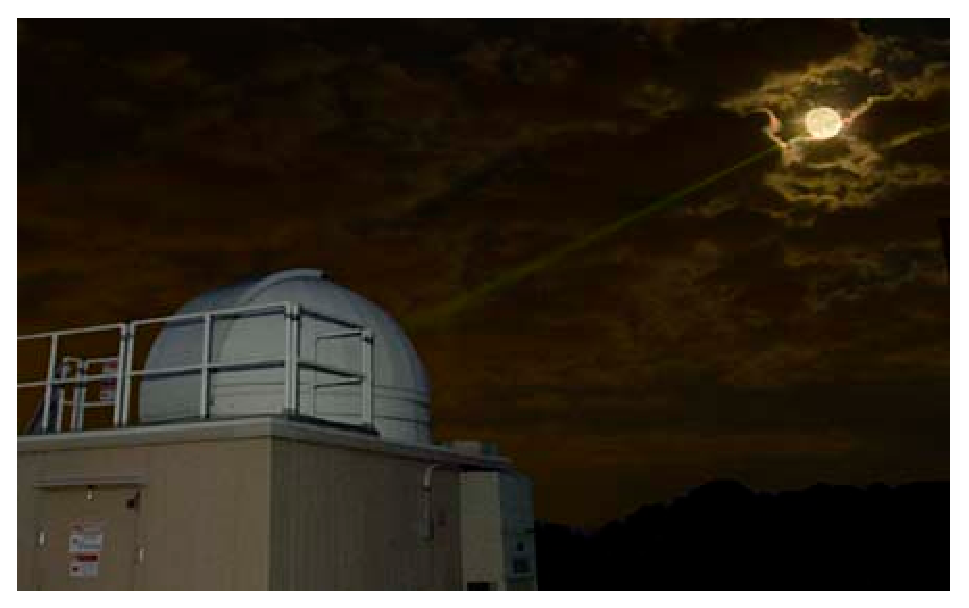
\includegraphics[width=.4\linewidth]{appendix_pomiary_laserowe.eps}
  \caption{}
  \label{fig:LLR_sub1}
\end{subfigure}%
\begin{subfigure}{.5\textwidth}
  \centering
  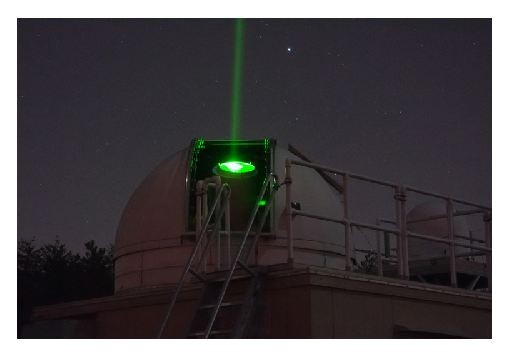
\includegraphics[width=.4\linewidth]{appendix_pomiary_laserowe2.eps}
  \caption{}
  \label{fig:LLR_sub2}
\end{subfigure}
\caption{\textit{Nocne pomiary do księzyca w obserwatorium NASA na stacji GGAO/GSFC w Greenbelt, Maryland, USA}
żródło: \protect\url{http://space-geodesy.gsfc.nasa.gov/multimedia/GeodesyNetwork/GeodesyNetworkImages.html}}
\label{fig:LLR_both}
\end{figure}

\section{Polski wkład}
\noindent Warto nadmienić, że w Borowcu niedaleko Poznania znajduje się obserwatorium astrogeodynamiczne Centrum Badań Kosmicznych Polskiej Akademii Nauk, 
w którym prowadzone są globalne i lokalne badania geodynamiczne z wykorzystaniem technik GPS oraz SLR.
W ramach obserwatorium działa także grupa Służby Czasu, która partycypuje w tworzeniu międzynarodowej skali czasu atomowego TAI oraz UTC.
Utrzymanie wysokiej dokładności pomiaru czasu (błąd jest obecnie mniejszy niż 2ns) ma kluczowe znaczenie w celu zapewnienia 
wysokiej dokładności pomiarów GNSS. \cite[][zakładka: infomrcje ogólne]{BOROWIEC}
\indent W ramach pomiarów SLR stacja badawcza w Borowcu prowadzi pomiary do kilkunastu sztucznych satlitów Zimi. 
W obserwarorium znajduje się także permanentna stacja IGS (jest zaangażowana w dostarczanie najwyższej jakości danych i wyników jako standardu dla Globalnego Systemu Nawigacji Satelitarnej) której odbiorniki zbierają obserwacje z satalitów GPS w sposób ciągły.
Permanentna stacja wchodzi w skład International GNSS service oraz EUREF. W ramach powyższych organizacji definiuje i realizuje Polski oraz Europejski Układ Odniesienia
\cite[][zakładka: Stacja IGS]{BOROWIEC}
 
